\chapter{General Discussion}\thumbforchapter
\newpage

\section{The phylotypic stage}

\begin{shadequote}[c]{George Box}
All models are wrong, but some are useful.
\end{shadequote}

While historically, the phylotypic stage has predominantly been examined and described through qualitative methods, the 21\textsuperscript{st} century started a paradigm shift towards a more quantitative and data-driven approach to understanding this phenomenon\cite{Chan2021}. The first notable quantitative investigation into the phylotypic stage was done by Bininda-Emonds \textit{et al.}, where they calculated temporal conservation as the order in which morphological embryonic features appear in vertebrates. However, it wasn't until the early 2010s that the field truly embraced quantitative methodologies with the simultaneous publication of two groundbreaking studies in Nature\cite{Kalinka2010, DomazetLoso2010}. In these works, Domazet-Lošo \textit{et al.} investigated the average developmental age of transcripts in \textit{D. rerio} and \textit{D. melanogaster}, whilst at the same time, Kalinka \textit{et al.} explored the temporal transcriptome similarities across different \textit{Drosophila} species. These molecular studies opened a new line of research to the quantitative basis of the phylotypic stage. The quantitative support for the phylotypic stage appeared stronger and stronger with each new study. So strong, that we quickly forget all the nonconforming studies.

The transcriptome age index (TAI), that Domazet-Lošo \textit{et al.} proposed, is the average transcript's evolutionary age calculated over time. The evolutionary age is defined as the number of taxonomic branches the gene dates back to. The idea of the TAI is that a temporal change is informative of more or less conservation. However, an independent re-analysis by Piasecka \textit{et al.} showed that due to major differences in transcript levels per gene, only a small subset of genes significantly influence the TAI\cite{Piasecka2013}. Log transforming the data, which is a standard processing step for this type of data, completely invalidates the results of the original study. One would ideally hope that this dependence of the results on transforming the data disqualifies the methodology, but the opposite appears to be true. The study that introduces the TAI is cited 88 times in the period between 2010-2013, and 359 times since the publication of Piasecka \textit{et al.} (years 2014-2023). As it turns out, you can now analyze the data with and without transformation, and keep the results that confirm your preferred hypothesis. An example of this is the study of Spiralian development by Wu \textit{et al.}\cite{Wu2019}, where they calculate the TAI on untransformed data for \textit{Crassostrea gigas}, \textit{Haliotis discus hannai} and \textit{Perinereis aibuhitensis}. Based on their results they claim that all three species show an inverse hourglass. The supplementary files, however, contain the TAI of \textit{Crassostrea gigas} after square root transformation, where the pattern changes from an inverse hourglass into a funnel. The  The authors practically ignore this result, and only conclude that at least it is not an hourglass-like pattern. Also worth mentioning is that the inverse hourglass pattern of \textit{Perinereis aibuhitensis} can be attributed to random noise. Where this study should be taken with a grain of salt, three influential evolutionary-developmental biologists (Pavel Tomanczak, Denis Duboule, and Andreas Hejnol) interact with each other on Twitter discussing this study and the implications for the universality of the hourglass model. Andreas Hejnol has authored two critical reviews of previous studies that claimed the phylotypic stage to be universal\cite{Dunn2018,hejnol2016}.

The Transcriptome Age Index (TAI), as introduced by Domazet-Lošo \textit{et al.}, is a metric of the average evolutionary age of transcripts over time\cite{DomazetLoso2010}. Evolutionary age is determined as the number of taxonomic branches to which a gene can be traced back. The central idea of the TAI is that temporal changes in gene expression provide insights into the degree of conservation during development. However, a re-analysis conducted by Piasecka \textit{et al.} raised some critical points\cite{Piasecka2013}. Their investigation revealed that the TAI is heavily influenced by a relatively small subset of genes due to major differences in transcript levels per gene (transcriptomic data is notoriously heteroscedastic). Log transforming the data, which is a standard processing step for this type of data, completely invalidates the results of the original study. One might expect such a dependency on data transformation to cast doubts on the method's reliability. Surprisingly, the opposite appears to be true. The original study introducing the TAI has been cited 88 times between 2010 and 2013, and 359 citations since Piasecka \textit{et al.}'s publication (covering the years 2014-2023). As it turns out, you can not analyze the data with and without transformation, and keep the results that reinforce your preferred hypothesis. A notable example of this is found in Wu \textit{et al.}'s study on Spiralian development\cite{Wu2019}. In their analysis of untransformed data for \textit{Crassostrea gigas}, \textit{Haliotis discus hannai}, and \textit{Perinereis aibuhitensis}, they claim to have found an inverse hourglass pattern. However, their supplementary data reveals a different pattern for \textit{Crassostrea gigas} after square root transformation, shifting from an inverse hourglass to a funnel shape. Remarkably, this crucial finding receives minimal attention in the study, with the authors merely stating that at least the transformed data does not show an hourglass-like pattern. Moreover, the transformed TAI of the other two time series are not even shown. It's also noteworthy that the inverse hourglass pattern of \textit{Perinereis aibuhitensis} can be attributed to random noise. Where this study should be taken with a grain of salt, it has sparked a discussion among three influential evolutionary-developmental biologists - Pavel Tomanczak, Denis Duboule, and Andreas Hejnol - on Twitter, about the universality of the hourglass model. It's worth mentioning that Andreas Hejnol has authored two critical reviews of previous studies that asserted the universality of the phylotypic stage\cite{Dunn2018,hejnol2016}.




The work of Barbara Piasecka, where she showed that the pattern of the TAI is caused by a subset of all genes was led by Marc Robinson-Rechavi. The main work of this study was not about the TAI, but about using a multitude of different metrics to estimate temporal evolutionary conservation. Their conclusion is that different metrics give different results. This is important, as perhaps (temporal) conservation is not that easy to measure, and/or depends on the methodology used. Marc Robinson-Rechavi in his later career, however, seems to have forgotten his earlier results and makes strong claims about the ortholog conjecture\cite{KryuchkovaMostacci2016} (methodological problems with this study were found\cite{Dunn2018}), and the hourglass model of conservation\cite{Liu2020,Liu2021,marletaz2018} (two of which I show have methodological problems in chapter XXX). 

In 2003 Bininda-Emonds \textit{et al.} showed an unexpected inverse hourglass on morphological rankings\cite{OlafRP2003}. Seventeen years later, Gerardo A. Cordero \textit{et al.} did a similar analysis of morphological timings across more species and morphological features\cite{Cordero2020}. To my knowledge, these are the only quantitative analyses of morphological characteristics with respect to the phylotypic stage. Cordero \textit{et al.} find the exact opposite of Bininda-Emonds \textit{et al.}; namely an hourglass pattern. Surprisingly, Cordero \textit{et al.} only comment that the difference between these two studies \textit{could} be caused by a difference in morphological characteristics, methodology, and species used, without further analysis of the differences. The main analysis of Bininda-Emonds \textit{et al.} is a mean-variance plot, something that takes 5 minutes to generate.

Levin \textit{et al.} suggested the transcriptomic inverse hourglass model as a method to distinguish different phyla in 2016\cite{Levin2016}. Their study has been rightfully criticized by Casey Dunn and Andreas Hejnol for the lack of a within-phylum control\cite{hejnol2016} and improper statistics\cite{Dunn2018}. For the size of the claim of a \textit{universal} phylotypic stage of high similarity within phyla, but low similarity between phyla, it is surprising they haven't addressed the criticism yet. Even more surprising, when a different group of evo-devo biologists investigated the transcriptome similarity between deuterostomes and the chordate amphioxus, which is a between phyla comparison, they found an hourglass-like pattern\cite{PerezPosada2022}. This is in direct contradiction to the inverse hourglass model of Levin \textit{et al}, but somehow receives no attention in their preprint. In chapter XXX I show that the transcriptomic inverse hourglass is a statistical artifact of normalization, and does not represent temporal conservation.

\begin{figure}[H]
    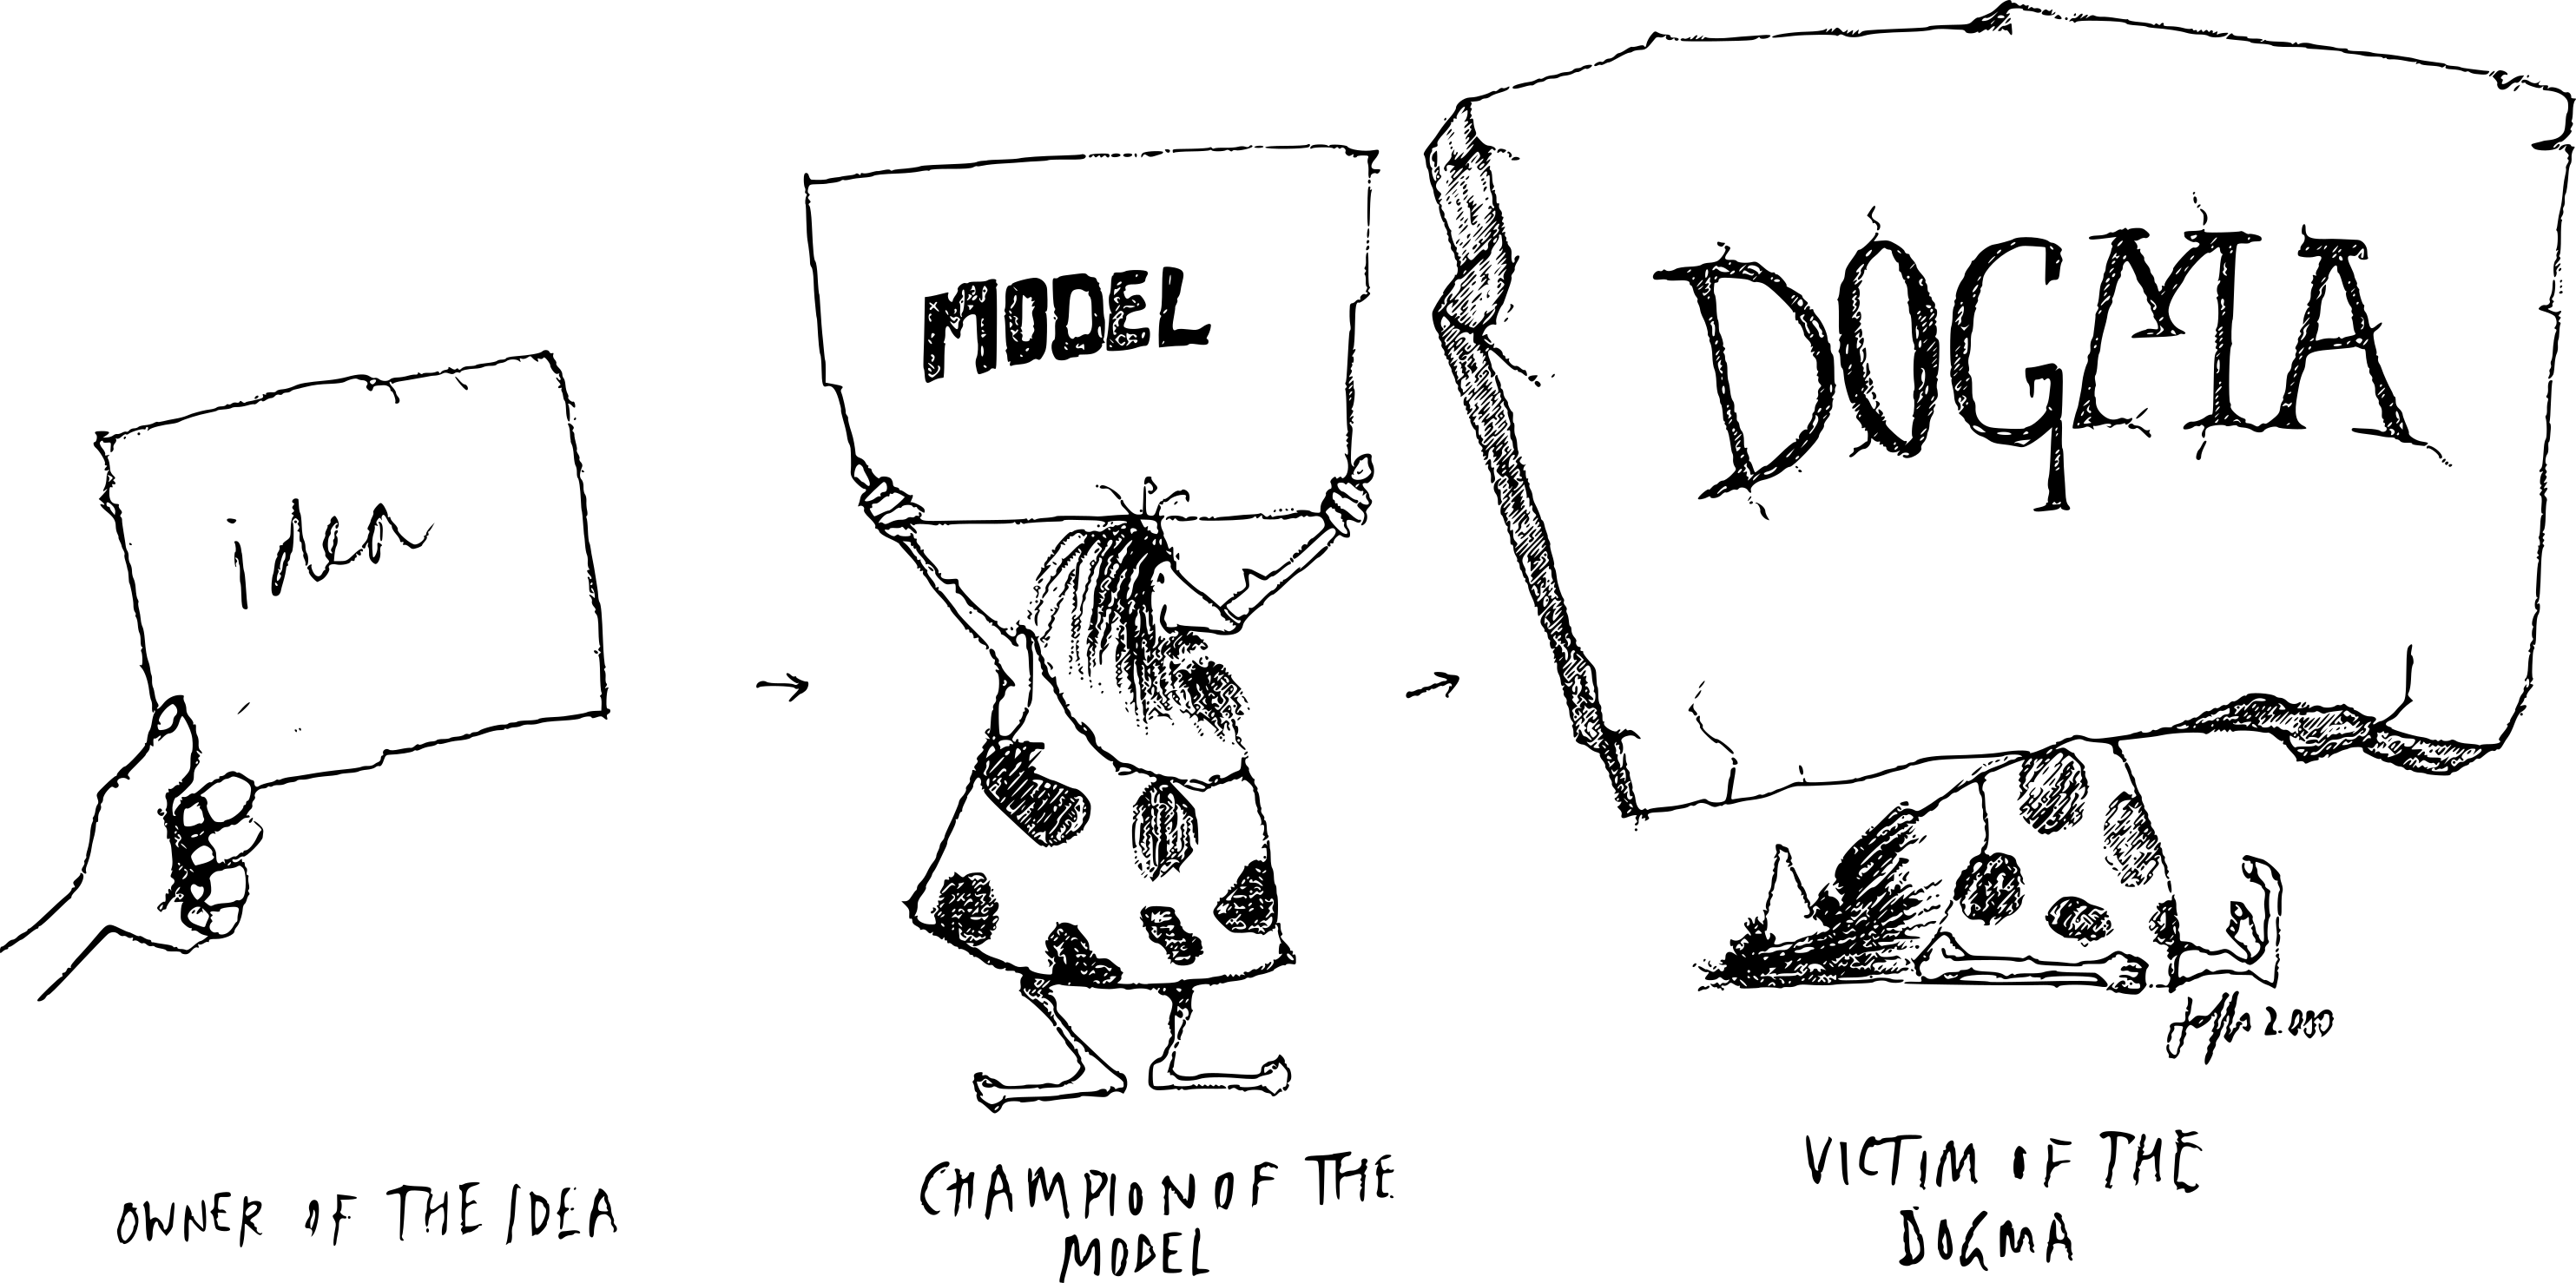
\includegraphics[width=\linewidth]{ch.discussion/imgs/dogma.png}
    \caption{\textbf{The phylotypic stage as a dogma} \cite{Caveman2000}.}
    \label{fig:dogma}
\end{figure}

Yoav Mayshar \textit{et al.} studied the phylotypic stage and the hourglass model from a single-cell point of view\cite{Mayshar2023}. They compare the proportions of different cell types between developing rabbit and mouse embryos. I show in chapter X that the mouse and rabbit time series are both discontinuous, and the temporal correlations between rabbit and mouse are heavily influenced by this. If anything, the discontinuous pattern in cell type proportions can be interpreted as a mid-developmental transition and as an inverse hourglass-like pattern. But somehow, Mayshar \textit{et al.} interpret this pattern as exactly the opposite, and claim that this is in confirmation of the hourglass model. How was this not caught by the reviewers of Cell, one of the most prestigious journals? When I asked Y. Mayshar on Twitter if their results perhaps represent an inverse hourglass, he commented with \say{this basically shows convergence of frequencies of cell states at \~e7.5-e8, preceding what would be normally considered as the phylotypic stage, though this is pretty vaguely defined...}. Pretty vague indeed.

There seems to be a certain level of apathy to genuinely understand, or even read, each other's work. Nearly all studies in the field contain obvious methodological problems, but they are treated as unimportant as long as these studies confirm your own prior beliefs. In chapter X and Y I show and discuss newly discovered problems with comparative approaches. I fear that highlighting these problems won't actually matter, as people will continue to believe their pet theories, and there will always be some methodology that in a way "confirms" it. For example, early in my PhD I met with one of the authors of the amphioxus paper, Ozren Bogdanovic. He is a staunch believer of the hourglass model, and even has a tattoo of it! I discussed some of my preliminary findings with him that the inverse hourglass is an artifact of normalization, and I expressed my concerns about the methodology they used in their analysis. His response was that he was not involved with the specific analysis, and as such saw no point in further discussing its potential problems. I'm still puzzled to this day why it is important who did an analysis for the validity of it. Similarly, a colleague in my department told me that even though I show that practically all quantitative methodologies used in the field are wrong, the fact remains that the phylotypic stage actually exists.

Based on my own re-analyses, it appears most methodologies actually support the null model. The null model for evolutionary embryonic development would be that there is no specific stage of higher or lower temporal conservation. The hourglass-like pattern between zebrafish and frogs based on transcriptomic correlations can be explained by within-species correlations alone. Similarly, the pattern of cell type proportion similarity between rabbits and mice, which is wrongfully called an hourglass, can be explained by discontinuous temporal sampling. Both the transcriptomic between-phyla inverse hourglass pattern and the morphological within-phylum inverse hourglass pattern are fully reproduced by simulated data with no specific temporal conservation. Only the \textit{Drosophila} enhancer conservation re-analysis results in a stage of maximum similarity, albeit a different point than the original authors find. Moreover, I simply do not agree with the methodological approach of this analysis. Taken together, there is little evidence to reject the null hypothesis of constant temporal conservation.

Furthermore, there is no consensus about what is actually expected to be conserved. The original observation that vertebrate embryos, perhaps, look more like each other at certain points in development than at other times, says nothing about the molecular basis for this. It has been quantitatively studied on the basis of embryonic lethality\cite{Uchida2018}, morphology\cite{OlafRP2003,Cordero2020}, DNA sequence conservation\cite{Piasecka2013,Quint2012,Liu2021} and activation order\cite{Uesaka2019}, cell type proportion\cite{Mayshar2023}, and whole-transcriptome similarity\cite{Piasecka2013,Irie2011,marletaz2018,Liu2020,Leong2021,PerezPosada2022,Kalinka2010}, with differing results. It begs the question of whether the wide adoption of transcriptomic methods is because we actually expect transcriptomic similarity based on (supposed) morphological similarity, or because transcriptomic methods are the most confirming of our prior beliefs that the phylotypic stage is the most conserved? Even when assuming the phylotypic stage to exist, why would we expect to be able to measure such a complex pattern with such crude methods as observational studies and whole embryo sequencing?

Historically, scientists have come up with the theories of taxonomic phyla and the phylotypic stage. But somehow along the way, these theories are now taken to be true, and require a molecular explanation. The root problem is that phyla and the phylotypic stage are loosely defined based on incidental observations, and do not make any predictions. As such, these ideas are unfalsifiable and by Popperian logic non-scientific. For example, animals are considered to be part of the same phylum if they share their basic body plan, but simultaneously the basic body plan is defined as the morphological characteristics shared by all animals of the same phyla\cite{BUDD2000}. The definition of the phylotypic stage is similarly ambiguous. Historically, the pharyngula stage\cite{https://doi.org/10.1093/icb/21.2.391}, early somite embryo\cite{ https://doi.org/10.1046/j.1420-9101.1993.6030457.x}, and the tail bud stage \cite{Slack1993} have all been proposed as the vertebrate phylotypic stage. The definition adhered to in quantitative studies in turn depends on which stage shows the highest quantitative conservation. For instance, the pharyngula \cite{Irie2011,marletaz2018}, the early somite embryo \cite{DomazetLoso2010}, or simply the stage(s) with the highest conservation metric\cite{Kalinka2010,Cordero2020} have all been named phylotypic stages in quantitative studies. Our current approach to studying the phylotypic stage, where we selectively include definitions and ignore nonconforming studies, is not only wrong but also not useful.

\section{scepia: gene regulatory networks}

Almost all gene regulatory approaches are context specific. But in the end a single set of instructions (DNA) for all contexts.

% \section{Do I regret seq2science?}

\section{The future of biology}

\subsection{Computational}

\subsection{lack of unified data encode like stuff}

For seq2science paper we tried paper X, Y, Z. DIFFICULT to get similar results.     

% No similarity between replicates:
% https://www.nature.com/articles/s41467-019-12687-4
% 
%  - drosophila sample missing and two other samples swapped
%  - inverse hourglass time orientation has negative values

NCBI sra is growing exponentially \cite{srawebsite}, but it is poorlymaintained.? It is an absolute pain to download from NCBI sra, hence sra-explorer, pysradb, fetchfastq, nf-core/fetchngs, and seq2science download-fastq workflow. Even more painful is that samples are submitted in non-standardized format. Need for MetaSRA and ALE. Works poorly, and is not necessary. Just properly add data. ENCOED is really nice

Single cell datasets often useless as only two out of three reads submitted. Single cell data is increasingly large.

Searat vs scanpy major differences in their log fold change calculation. How is this allowed?

\subsection{Open Science}



\subsection{Too much descriptive, not enough understanding}

Early adopters have been overwhelmed by the size of the data, lack of analytical tools, but mostly the number of different cell types generating a flurry of research articles with titles like "single cell sequencing in tissue X reveals heterogeneity".  

\subsection{Move away from mRNA}

mRNA and protein relation.
The correlation between protein expression and mRNA expression seems high (0.87) measured across cell types. However, genes with high protein expression generally have high mRNA expression. So it is easy to get high prediction. If you want to predict a single gene you get correlation of 0.41. Simpson's paradox! 
https://www.nature.com/articles/nature23293

https://www.biorxiv.org/content/10.1101/2023.05.23.541948v1

cool work of michael levine on xenobots

% https://twitter.com/nimwegenlab/status/1671923176626847744?s=12&t=oyB_faiBr8aHqHcjXZE50A

\begin{figure}[H]
    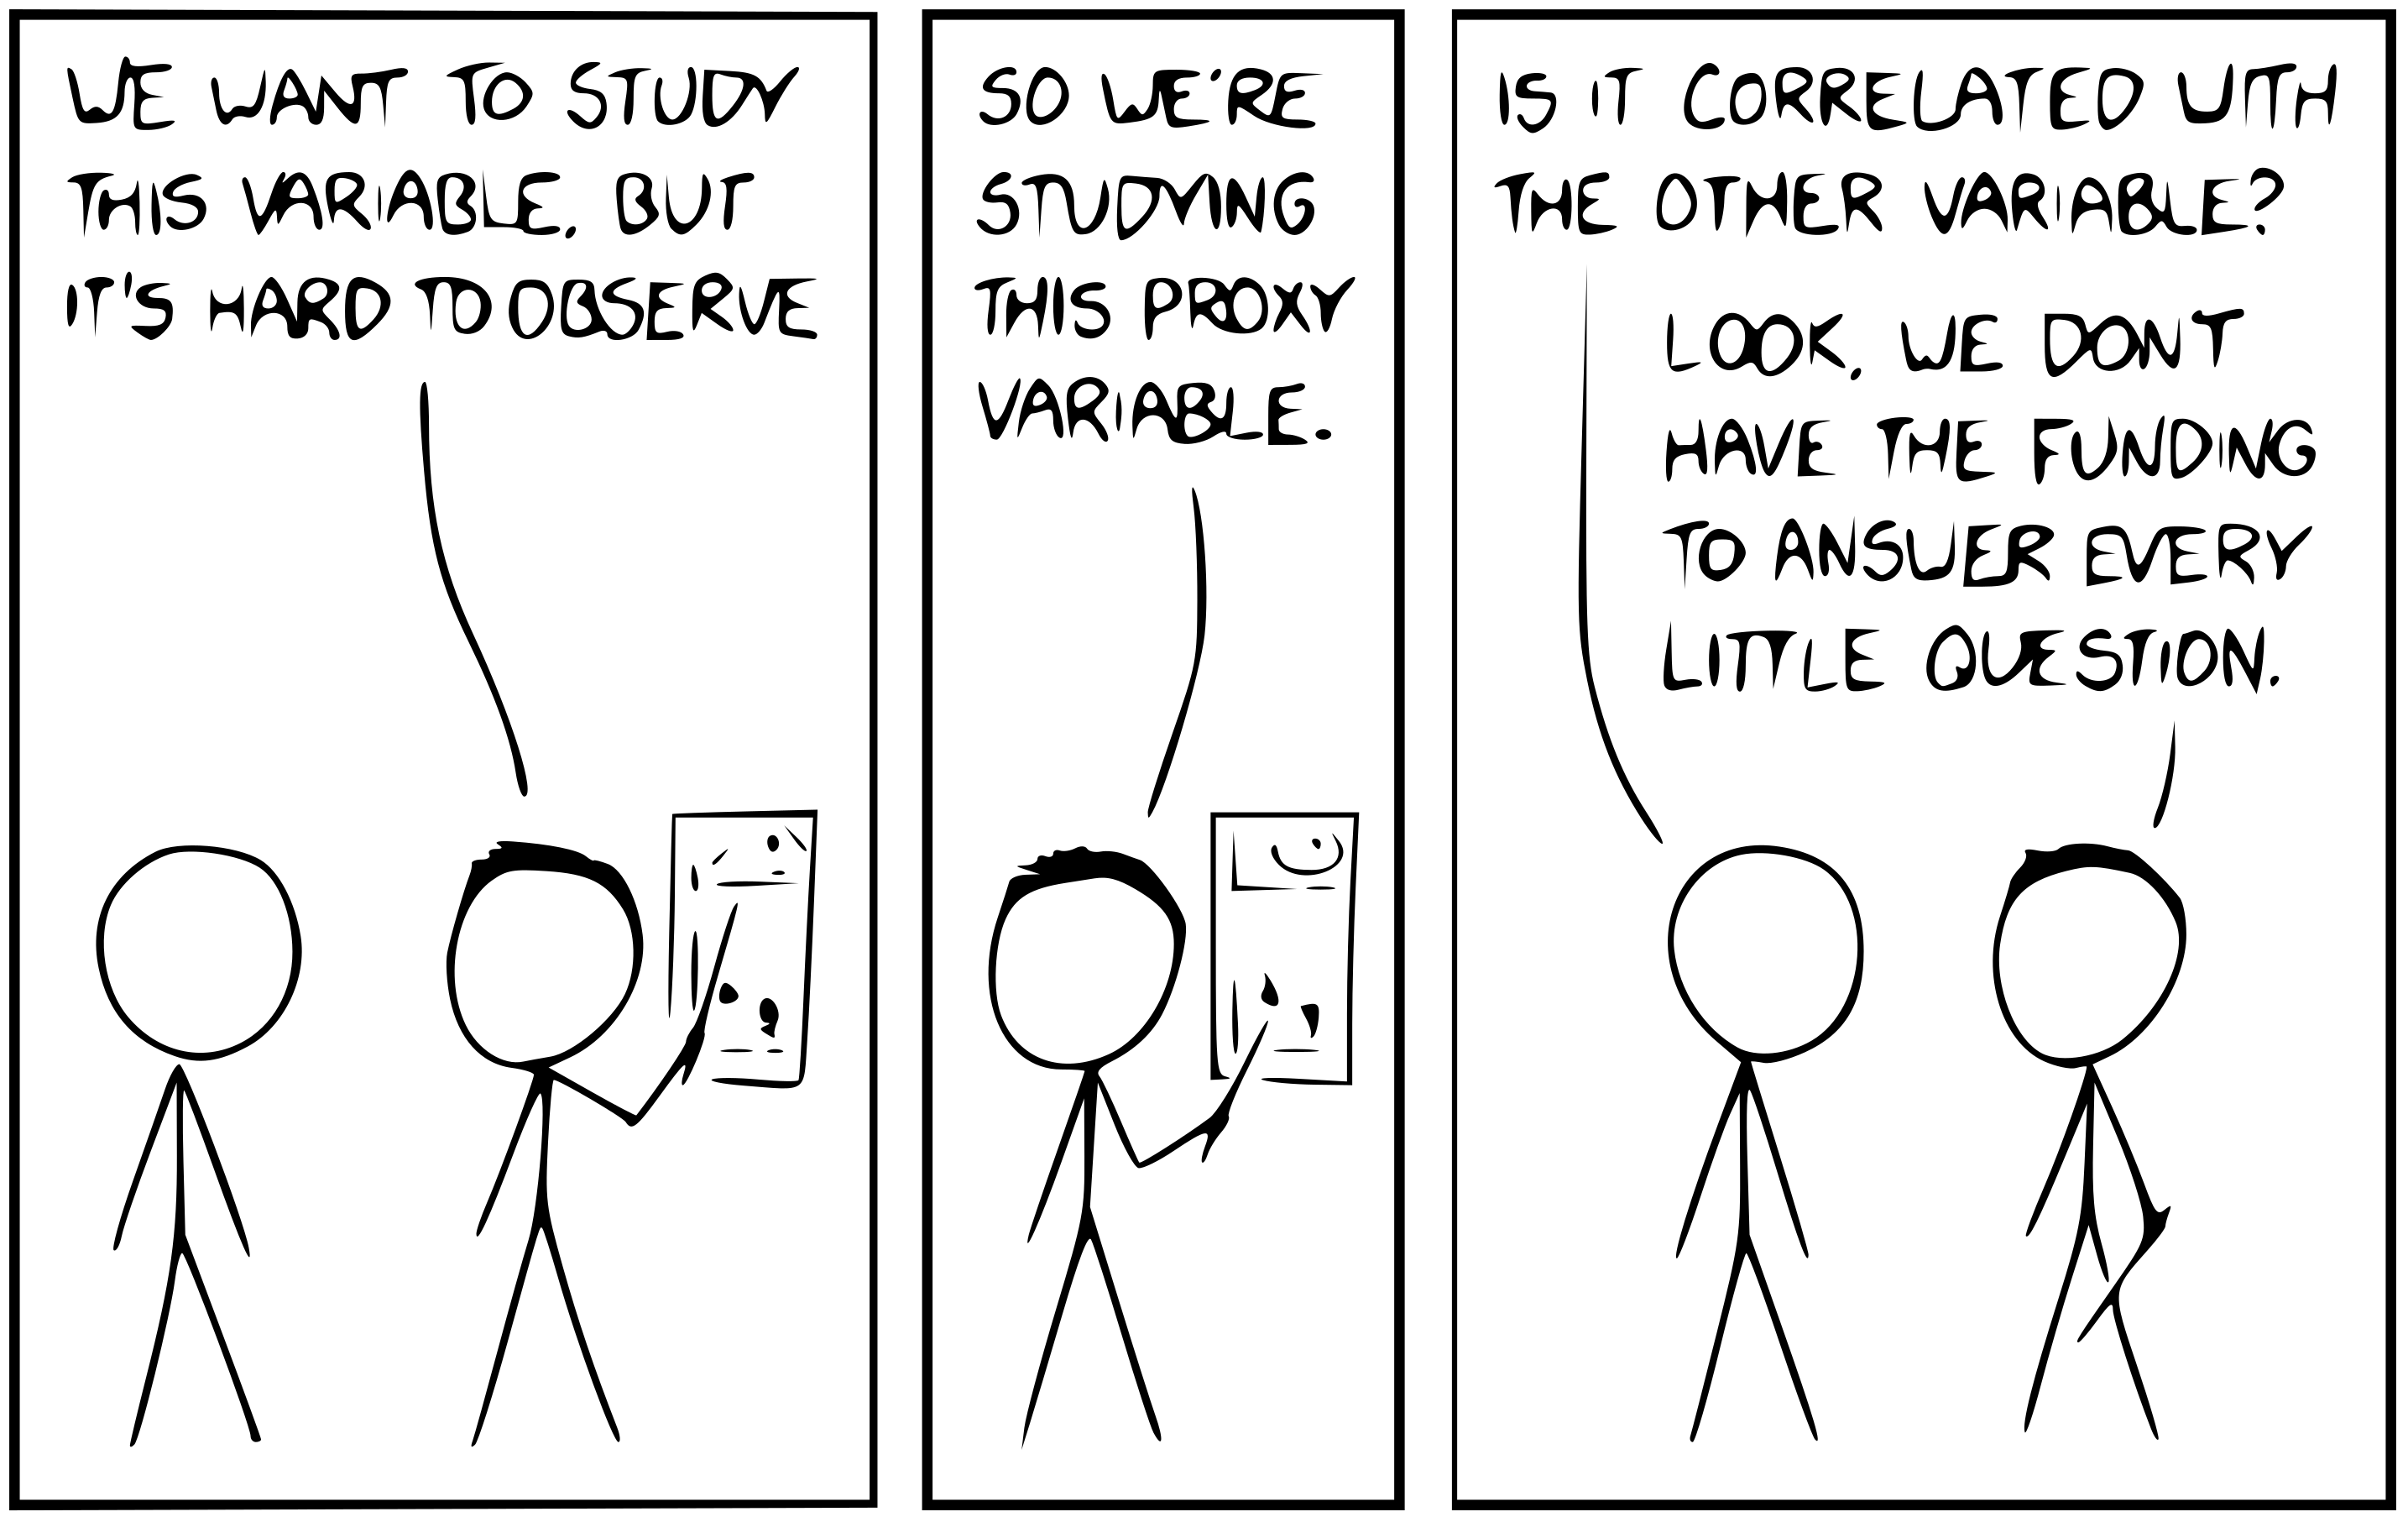
\includegraphics[width=\linewidth]{ch.discussion/imgs/xkcd.png}
    \caption{\textbf{xkcd}. URL: https://xkcd.com/2652}
    \label{fig:xkcd}
\end{figure}

% \subsection{Stop blaming "the incentives"}

% incentives: https://www.talyarkoni.org/blog/2018/10/02/no-its-not-the-incentives-its-you/

\subsection{Self-correcting}

e.g. wild growth covid papers

papers keep on being cited after retraction or criticism. Number one paper of percentage of genome is functional gives highly criticized ENCODE paper.

highlight cancer microbiome paper: https://www.nature.com/articles/s41586-020-2095-1. And the negative result : https://www.biorxiv.org/content/10.1101/2023.07.28.550993v1.full.pdf

comparison of mouse vs human transcriptome: https://www.pnas.org/doi/full/10.1073/pnas.1413624111 and the re-analysis that they were wrong: https://f1000research.com/articles/4-121/v1

ENCODE claiming 80\% biochemical and criticism on it. When googling first result is ENCODE (I think)

Our golden standard is actual clinical trials! Our methods don't seem to work so well..?
https://www.ncbi.nlm.nih.gov/pmc/articles/PMC6409418/
https://journals.plos.org/plosmedicine/article?id=10.1371/journal.pmed.0020124

% Biology is messy, but that does not mean computational biology has to be.
